\subsection{Monthly Revenue Trends}
This visualization compares monthly revenue trends across product categories to identify changes in category-level performance over time. Both a category name slicer and a timeline slicer were incorporated to support filtering and trend analysis.
\begin{lstlisting}[language=SQL]
SELECT Month, SUM(SalesRevenue) AS TotalRevenue
FROM Sales
GROUP BY Month
ORDER BY Month;
\end{lstlisting}

\textbf{Visualization:}
\begin{center}
    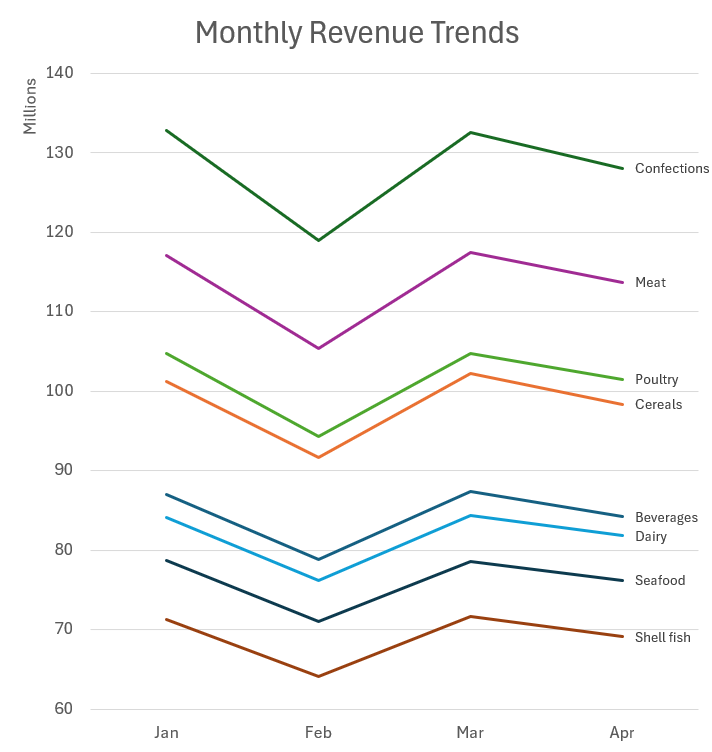
\includegraphics[width=1\linewidth]{Images/7.CHART_monthly-revenue-trends.png}
\end{center}
